\subsection{Интерполяционные полиномы}

\subsubsection{Многочлен Лагранжа}

\subsubsubsection{Узловые базисные функции}

Рассмотрим функцию $f(\xi)$, заданную в области $D$.
Внутри этой области зададим $N$ узловых
точек $\xi_i, i=\overline{0,N-1}$.
Приближение функции $f$ будем искать в виде
\begin{equation}
\label{eq:nodal_basis}
f(\xi) \approx \sum_{i=0}^{N-1} f_i \phi_i(\xi),
\end{equation}
где  $f_i = f(\xi_i)$, $\phi_i$ -- узловая базисная функция.
Потребуем, чтобы это выражение выполнялось точно для всех
заданных узлов интерполяции $\xi = \xi_i$. Тогда, исходя из определения \cref{eq:nodal_basis}, запишем условие 
на узловую базисную функцию
\begin{equation}
\label{eq:nodal_bases_conditions}
\phi_i(\xi_j) = 
\begin{cases}
1, &\quad i = j, \\
0, &\quad i \neq j.
\end{cases}
\end{equation}
Дополнительно потребуем, чтобы формула \cref{eq:nodal_basis} была
точной для постоянных функций
$$
f(\xi)=\const \hence f_i = \const.
$$
Тогда для любого $\xi$ должно выполняться условие
\begin{equation}
\label{eq:nodal_bases_unitsum}
\sum_{i=0}^{N-1} \phi_i(\xi) = 1, \qquad \xi \in D.
\end{equation}

Задача построения интерполяционной функции состоит
в конкретном определении узловых базисов
$\phi_i(\xi)$ по заданному набору
узловых точек $\xi_i$ и значениям
функции в них $f_i$. Будем искать базисы
в виде многочленов вида
\begin{equation}
\label{eq:nodal_basis_1d_decomp}
\phi_i(\xi) = \sum_{a} A_i^{(a)} \xi^{a} =
A_i^{(0)} + 
A_i^{(1)} \xi + 
A_i^{(2)} \xi^2 +  \ldots, \qquad i = \overline{0, N-1}.
\end{equation}
Определять коэффициенты $A^{(a)}_i$ будем из условий \cref{eq:nodal_bases_conditions},
которое даёт $N$ линейных уравнений относительно неизвестных $A_i^{(a)}$ для каждого $i=\overline{0, N-1}$.
Таким образом, в выражениях \cref{eq:nodal_basis_1d_decomp} должно быть
ровно $N$ слагаемых.
Будем использовать последовательный набор степеней: $a=\overline{0,N-1}$.
Выпишем систему линейных уравнений для $0$-ой базисной функции
\begin{equation*}
\begin{aligned}
& \phi_0(\xi_0) = A_0^{(0)} + A_0^{(1)} \xi_0 + A_0^{(2)} \xi_0^2 + A_0^{(3)} \xi_0^3 + \ldots = 1, \\
& \phi_0(\xi_1) = A_0^{(0)} + A_0^{(1)} \xi_1 + A_0^{(2)} \xi_1^2 + A_0^{(3)} \xi_1^3 + \ldots = 0, \\
& \phi_0(\xi_2) = A_0^{(0)} + A_0^{(1)} \xi_2 + A_0^{(2)} \xi_2^2 + A_0^{(3)} \xi_2^3 + \ldots = 0, \\
& \ldots
\end{aligned}
\end{equation*}
или в матричном виде
\begin{equation*}
\left(
\begin{array}{ccccc}
1 & \xi_0 & \xi_0^2 & \xi_0^3 & \ldots \\[5pt]
1 & \xi_1 & \xi_1^2 & \xi_1^3 & \ldots \\[5pt]
1 & \xi_2 & \xi_2^2 & \xi_2^3 & \ldots \\[5pt]
1 & \xi_3 & \xi_3^2 & \xi_3^3 & \ldots \\[5pt]
\ldots &&&&
\end{array}
\right)
\left(
\begin{array}{c}
A_0^{(0)} \\[5pt]
A_0^{(1)} \\[5pt]
A_0^{(2)} \\[5pt]
A_0^{(3)} \\[5pt]
\vdots
\end{array}
\right)
=
\left(
\begin{array}{c}
1 \\[5pt]
0 \\[5pt]
0 \\[5pt]
0 \\[5pt]
\vdots
\end{array}
\right)
\end{equation*}
Записывая аналогичные выражения для остальных базисных функций, получим систему матричных уравнений
вида $C A = E$:
\begin{equation*}
\left(
\begin{array}{ccccc}
1 & \xi_0 & \xi_0^2 & \xi_0^3 & \ldots \\[5pt]
1 & \xi_1 & \xi_1^2 & \xi_1^3 & \ldots \\[5pt]
1 & \xi_2 & \xi_2^2 & \xi_2^3 & \ldots \\[5pt]
1 & \xi_3 & \xi_3^2 & \xi_3^3 & \ldots \\[5pt]
\ldots &&&&
\end{array}
\right)
\left(
\begin{array}{ccccc}
A_0^{(0)} & A_1^{(0)} & A_2^{(0)} & A_3^{(0)} & \ldots\\[5pt]
A_0^{(1)} & A_1^{(1)} & A_2^{(1)} & A_3^{(1)} &       \\[5pt]
A_0^{(2)} & A_1^{(2)} & A_2^{(2)} & A_3^{(2)} &       \\[5pt]
A_0^{(3)} & A_1^{(3)} & A_2^{(3)} & A_3^{(3)} &       \\[5pt]
\vdots
\end{array}
\right)
=
\left(
\begin{array}{ccccc}
1 & 0 & 0 & 0 & \ldots \\[5pt]
0 & 1 & 0 & 0 &        \\[5pt]
0 & 0 & 1 & 0 &        \\[5pt]
0 & 0 & 0 & 1 &        \\[5pt]
\vdots
\end{array}
\right)
\end{equation*}
Отсюда матрица неизвестных коэффициентов $A$ определится как
\begin{equation}
\label{eq:nodal_basic_amat}
A = C^{-1} = 
\left(
\begin{array}{ccccc}
1 & \xi_0 & \xi_0^2 & \xi_0^3 & \ldots \\[5pt]
1 & \xi_1 & \xi_1^2 & \xi_1^3 & \ldots \\[5pt]
1 & \xi_2 & \xi_2^2 & \xi_2^3 & \ldots \\[5pt]
1 & \xi_3 & \xi_3^2 & \xi_3^3 & \ldots \\[5pt]
\ldots &&&&
\end{array}
\right) ^{-1}.
\end{equation}

Подставляя полином \cref{eq:nodal_basis_1d_decomp} в условие согласованности \cref{eq:nodal_bases_unitsum},
получим требование
\begin{equation*}
\sum_{i=0}^{N-1} A_i^{(a)} = 
\begin{cases}
1, \quad a=0, \\
0, \quad a=\overline{1,N-1}.
\end{cases}
\end{equation*} 
То есть сумма всех свободных членов в интерполяционных полиномах должна
быть равна единице, а сумма коэффициентов при остальных степенях -- нулю.
Можно показать, что это свойство выполняется для любой матрицы $A=C^{-1}$,
в случае, если первый столбец матрицы $C$ состоит из единиц.
То есть условие согласованности требует наличие свободного члена
с интерполяционном полиноме.


\subsubsubsection{Интерполяция в параметрическом отрезке}
\label{sec:segment_bases}
Будем рассматривать область интерполяции $D=[-1, 1]$.
В качестве первых двух узлов интерполяции возьмем границы области:
$\xi_0 = -1$, $\xi_1 = 1$.
\paragraph{Линейный базис}
Будем искать интерполяционный базис в виде
$$
\phi_i(\xi) = A_i^{(0)} + A_i^{(1)} \xi.
$$
на основе двух условий:
$$
\phi_i(-1) = A_i^{(0)} - A_i^{(1)} = \delta_{0i}, \quad \phi_i(1) = A_i^{(0)} + A_i^{(1)}\delta_{1i}.
$$
Составим матрицу $C$, записав эти условия в матричном виде
$$
C =
\left(
\begin{array}{l|rr}
      & A^{(0)} & A^{(1)}\\
\hline
\phi(-1) & 1 & -1 \\[5pt]
\phi(1) & 1 &  1 \\[5pt]
\end{array}
\right)
$$
и, согласно \cref{eq:nodal_basic_amat}, найдём матрицу коэффициентов
$$
A =
\left(
\begin{array}{cc}
A_0^{(0)} & A_1^{(0)} \\[5pt]
A_0^{(1)} & A_1^{(1)} \\[5pt]
\end{array}
\right) = C^{-1} =
\left(
\begin{array}{l|rr}
     & \phi_0   & \phi_1  \\
\hline
1    & \frac12  & \frac12 \\[5pt]
\xi  & -\frac12 & \frac12 \\[5pt]
\end{array}
\right).
$$
Отсюда узловые базисные функции примут вид (\figref{fig:basis1d_linear})
\begin{equation}
\label{eq:segment_linear_basis}
\begin{aligned}
&\phi_0(\xi) = \frac{1 - \xi}{2}, \\
&\phi_1(\xi) = \frac{1 + \xi}{2}.
\end{aligned}
\end{equation}
Окончательно интерполяционная функция из определения \cref{eq:nodal_basis}
примет вид
$$
f(\xi) \approx \frac{1 - \xi}{2} f(-1) + \frac{1 + \xi}{2} f(1).
$$
\begin{figure}[h!]
\centering
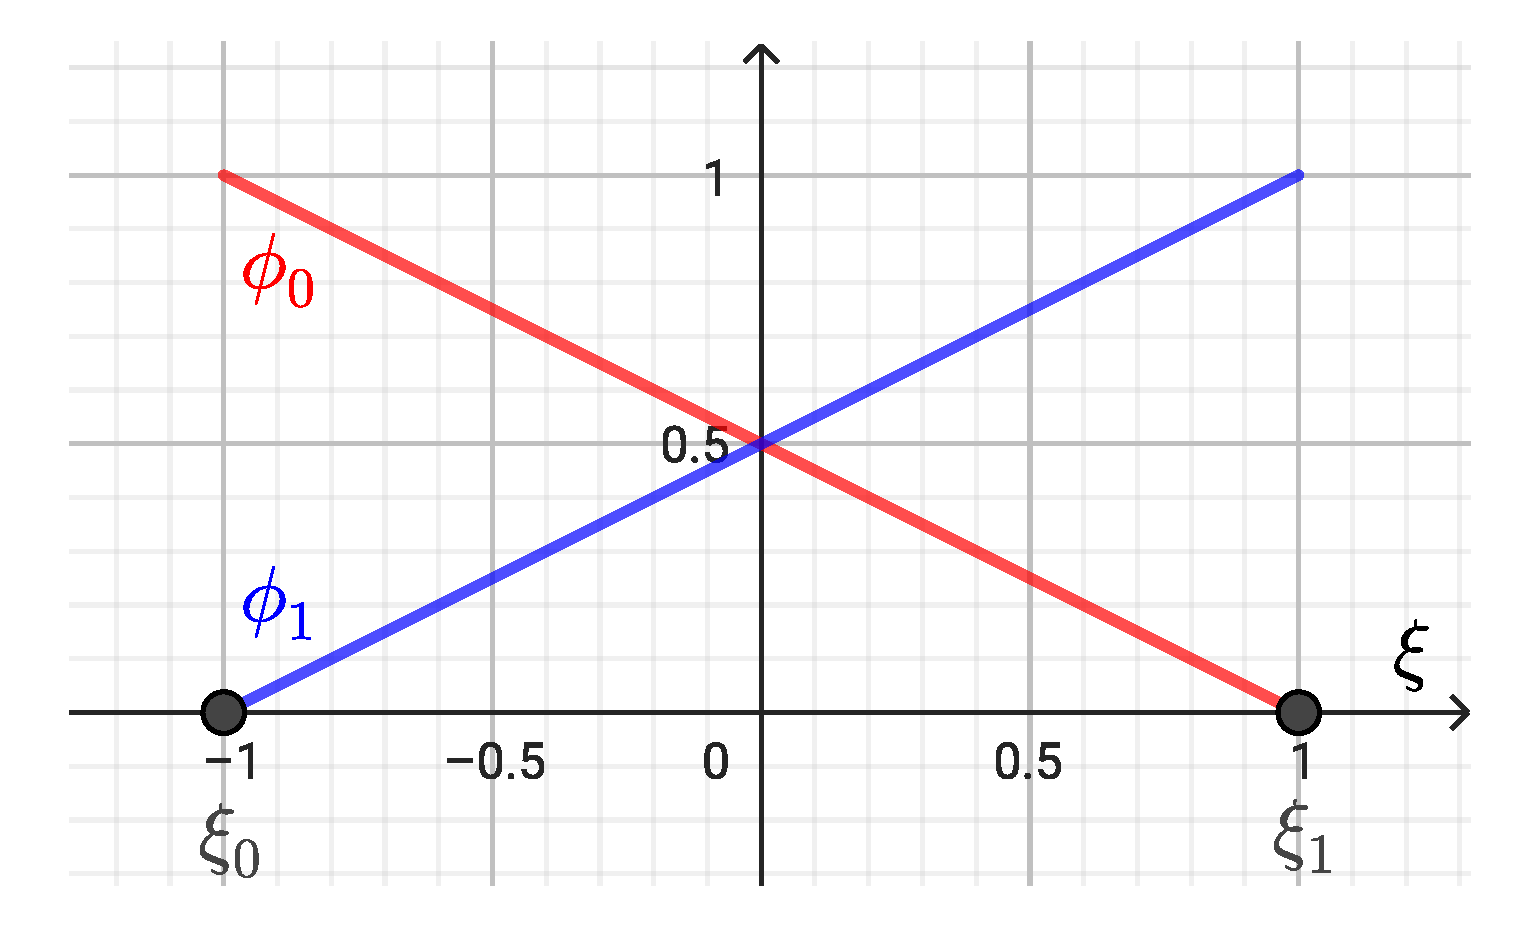
\includegraphics[width=0.4\linewidth]{basis1d_linear.pdf}
\caption{Линейный базис в параметрическом отрезке}
\label{fig:basis1d_linear}
\end{figure}

\paragraph{Квадратичный базис}
Будем искать интерполяционный базис в виде
$$
\phi_i(\xi) = A_i^{(0)} + A_i^{(1)} \xi + A_i^{(2)} \xi^2.
$$
По сравнению с линейным случаем, в форму базиса добавился ещё один неизвестый коэффициент $A_i^{(2)}$,
поэтому в набор условий \cref{eq:nodal_bases_conditions} требуется ещё одно уравнение (ещё одна узловая точка).
Поместим её в центр параметрического сегмента $\xi_2 = 0$. Далее будем действовать по
аналогии с линейным случаем:
$$
C = \left(
\begin{array}{l|rrr}
         &  A^{(0)} & A^{(1)}   & A^{(2)} \\ 
\hline
\phi(-1) & 1 & -1 & 1\\[5pt]
\phi(1)  & 1 &  1 & 1\\[5pt]
\phi(0)  & 1 &  0 & 0
\end{array}
\right)
\hence
A = C^{-1} = \left(
\begin{array}{l|rrr}
       & \phi_0   & \phi_1   & \phi_2 \\
\hline
 1     & 0        &  0       &  1     \\[5pt]
 \xi   & -\frac12 &  \frac12 &  0     \\[5pt]
 \xi^2 &  \frac12 &  \frac12 & -1     \\[5pt]
\end{array}
\right).
$$
Узловые базисные функции для квадратичной интерполяции примут вид (\figref{fig:basis1d_quadratic})
\begin{equation}
\label{eq:segment_quadratic_basis}
\begin{aligned}
&\phi_0(\xi) = \frac{\xi^2 - \xi}{2}, \\
&\phi_1(\xi) = \frac{\xi^2 + \xi}{2}, \\
&\phi_2(\xi) = 1 - \xi^2.
\end{aligned}
\end{equation}

\begin{figure}[h!]
\centering
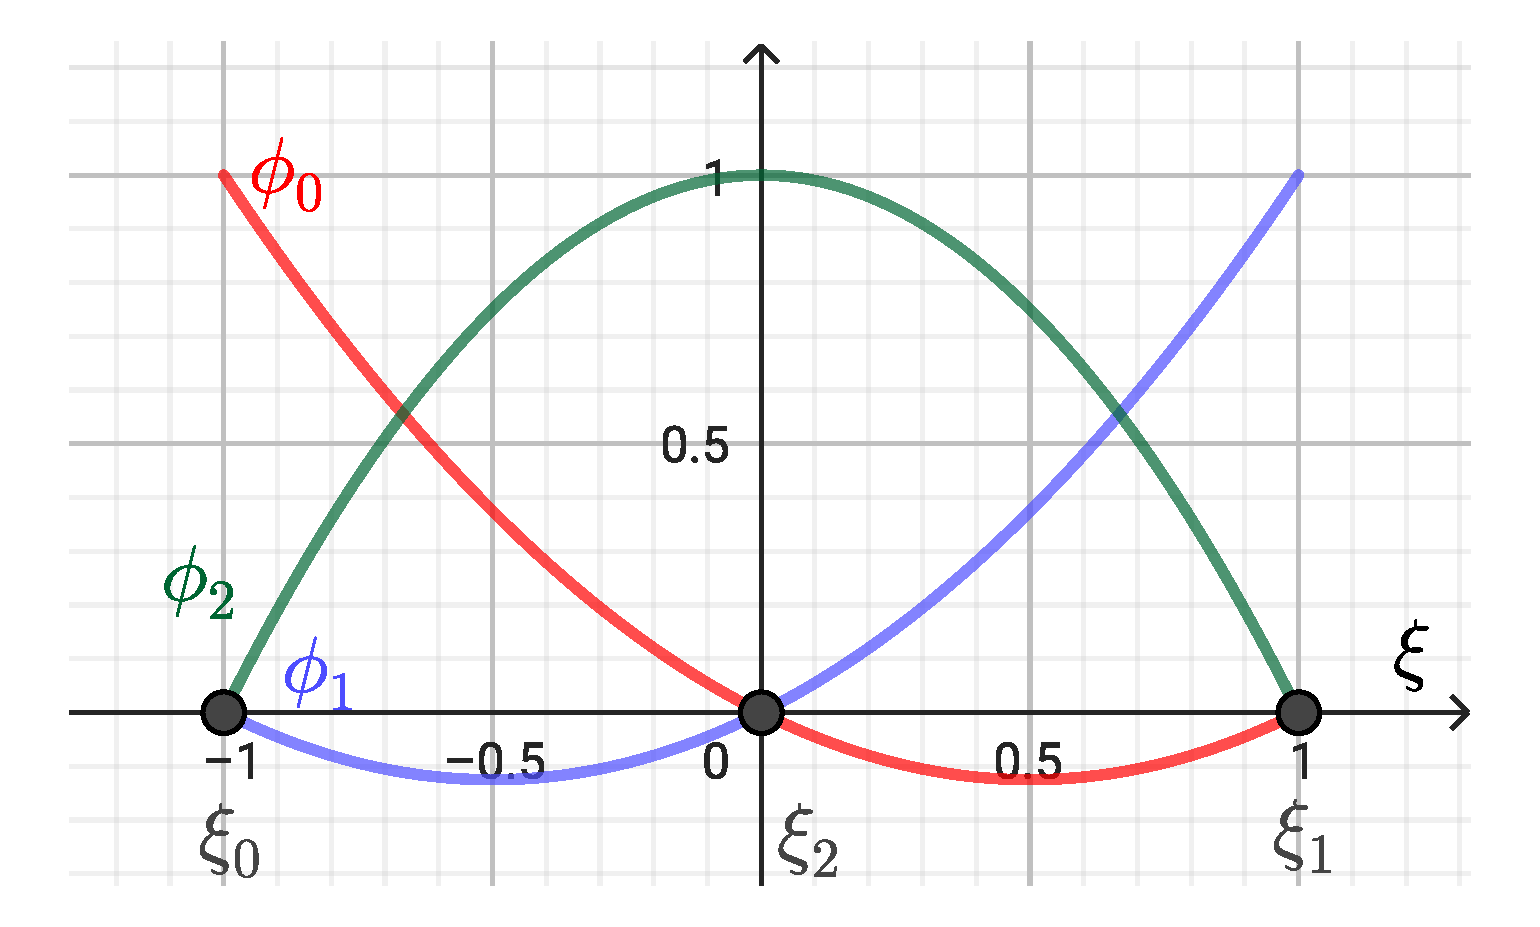
\includegraphics[width=0.4\linewidth]{basis1d_quadratic.pdf}
\caption{Квадратичный базис в параметрическом отрезке}
\label{fig:basis1d_quadratic}
\end{figure}

\paragraph{Кубический базис}
Интерполяционный базис будет иметь вид
$$
\phi_i(\xi) = A_i^{(0)} + A_i^{(1)} \xi + A_i^{(2)} \xi^2 + A_i^{(3)} \xi^3.
$$
Для нахождения четырёх коэффициентов нам понадобится четыре узла интерполяции.
Две из них -- это границы параметрического отрезка. Остальные две разместим
так, чтобы разбить отрезок на равные интервалы:
$\xi_2 = -\tfrac13$, $\xi_3 = \tfrac13$.
Далее вычислим матрицу коэффициентов:
$$
C =
\left(
\begin{array}{l|rrrr}
                &  A^{(0)}  &  A^{(1)}      & A^{(2)}     & A^{(3)}         \\
\hline
\phi(-1)        &  1  & -1        & 1         &  -1           \\[5pt]
\phi( 1)        &  1  & 1         & 1         &   1           \\[5pt]
\phi(-\tfrac13) &  1  & -\tfrac13 & \tfrac19  &  -\tfrac1{27} \\[5pt]
\phi(\tfrac13)  &  1  &  \tfrac13 & \tfrac19  &   \tfrac1{27}
\end{array}
\right)
\hence
A = C^{-1} =
\frac{1}{16}
\left(
\begin{array}{l|rrrr}
      & \phi_0 & \phi_1 & \phi_2 & \phi_3 \\
\hline
1     & -1     & -1     &   9    &  9     \\[5pt]
\xi   &  1     & -1     & -27    &  27    \\[5pt]
\xi^2 &  9     &  9     & -9     & -9     \\[5pt]
\xi^3 & -9     &  9     &  27    & -27   
\end{array}
\right)
$$
Узловые базисные функции для квадратичной интерполяции примут вид (\figref{fig:basis1d_cubic})
\begin{equation}
\label{eq:segment_cubic_basis}
\begin{aligned}
&\phi_0(\xi) = \frac{1}{16}\left(-1 + \xi + 9 \xi^2 -9 \xi^3\right), \\
&\phi_1(\xi) = \frac{1}{16}\left(-1 - \xi + 9 \xi^2 +9 \xi^3\right), \\
&\phi_2(\xi) = \frac{1}{16}\left(9 -27 \xi - 9\xi^2 + 27 \xi^3\right), \\
&\phi_3(\xi) = \frac{1}{16}\left(9 +27 \xi - 9\xi^2 - 27 \xi^3\right), \\
\end{aligned}
\end{equation}

\begin{figure}[h!]
\centering
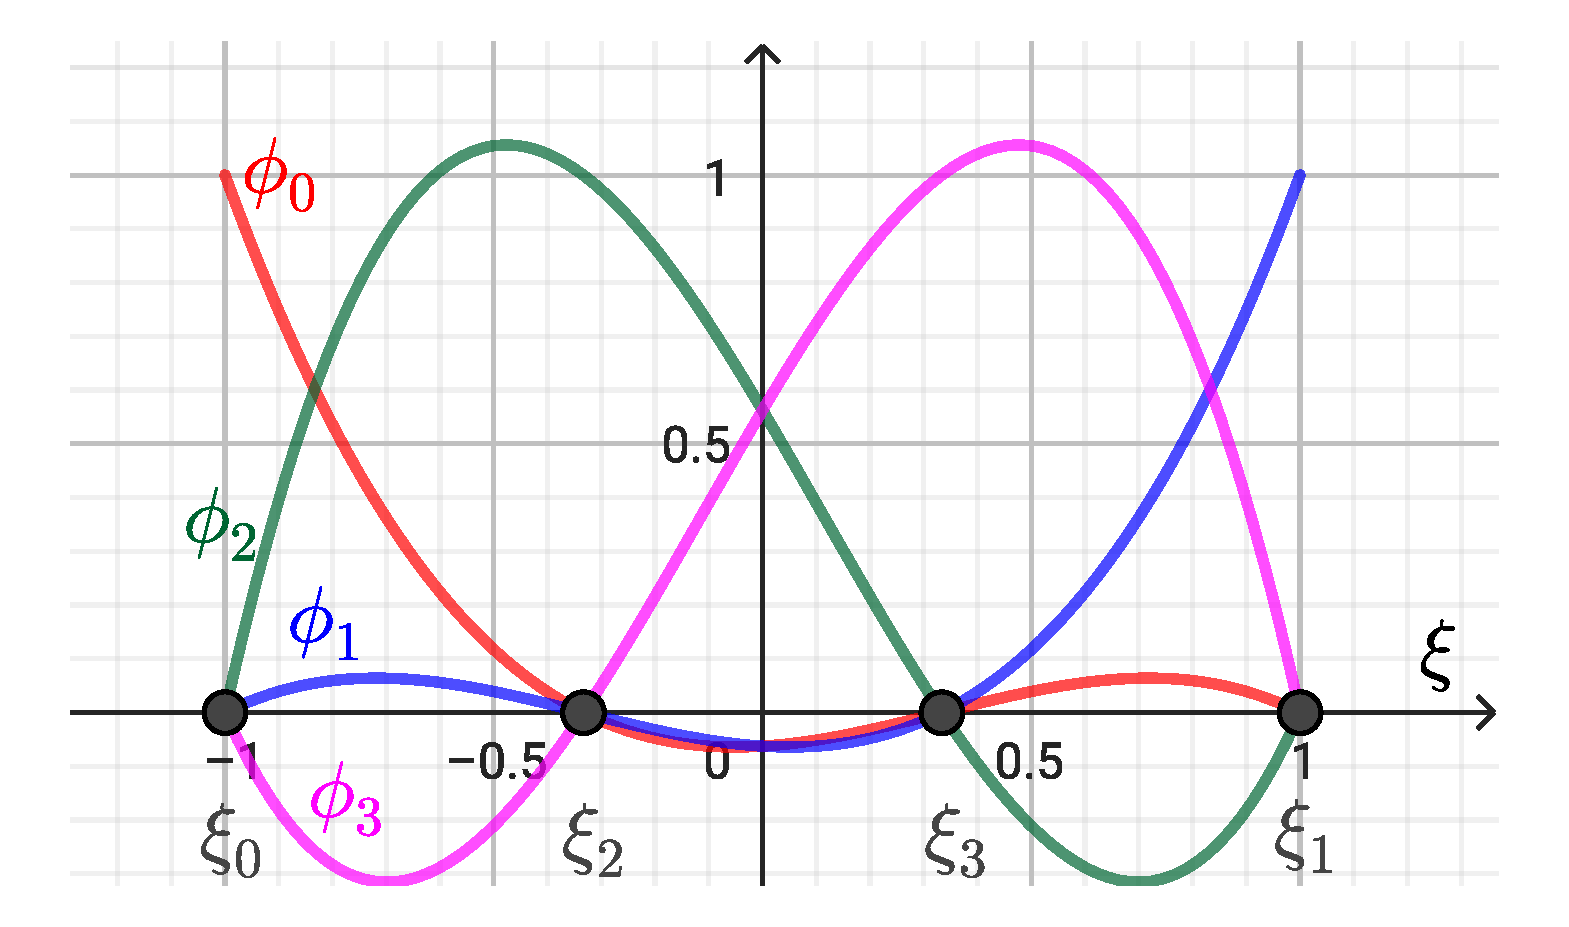
\includegraphics[width=0.4\linewidth]{basis1d_cubic.pdf}
\caption{Кубический базис в параметрическом отрезке}
\label{fig:basis1d_cubic}
\end{figure}

На \figref{fig:basis1d_compare} представлено сравнение результатов
аппроксимации функции $f(x) = -x + \sin(2 x + 1)$ линейным, квадратичным и кубическим базисом.
Видно, что все интерполяционные приближения точно попадают в функцию в своих
узлах интерполяции, а между узлами происходит аппроксимация полиномом соответствующей степени.

\begin{figure}[h!]
\centering
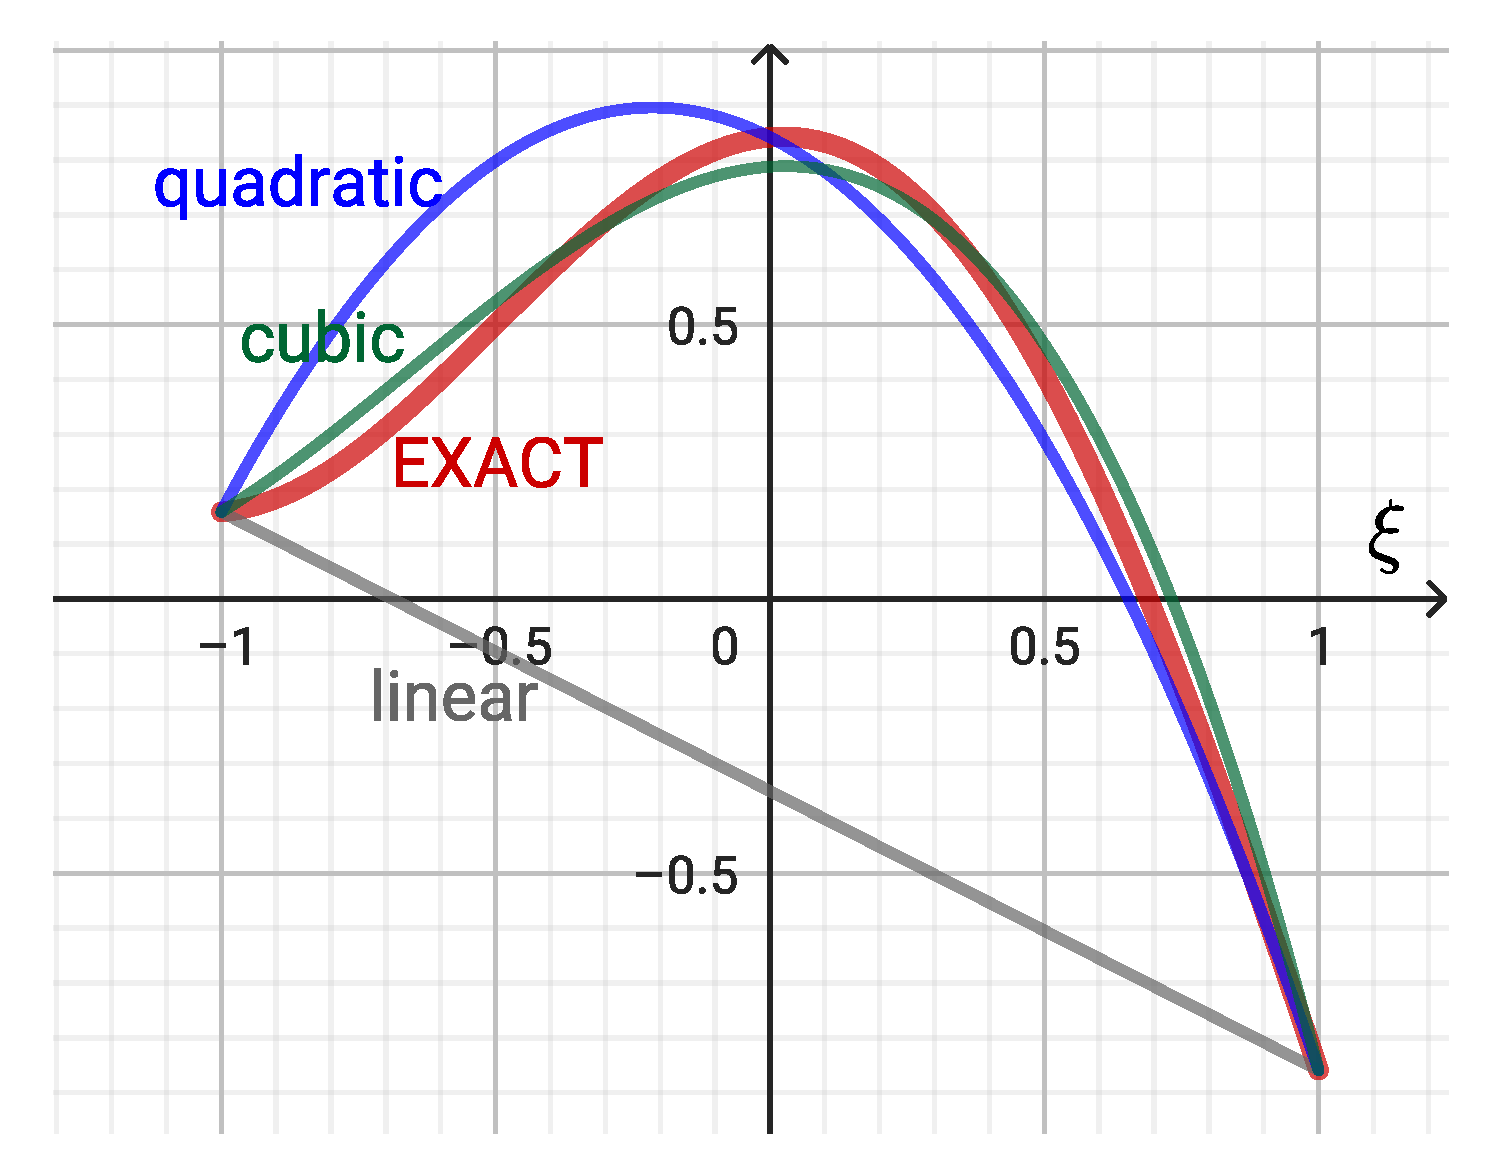
\includegraphics[width=0.4\linewidth]{basis1d_compare.pdf}
\caption{Результат интерполяции}
\label{fig:basis1d_compare}
\end{figure}

\subsubsubsection{Интерполяция в параметрическом треугольнике}
\label{sec:triangle_bases}
Теперь рассмотрим двумерное обобщение формулы
\begin{figure}[h!]
\centering
\includegraphics[width=0.5\linewidth]{triangle_basis_points.pdf}
\caption{Расположение узловых точек в параметрическом треугольнике. а) линейный базис, б) квадратичный базис, в) кубический базис, г) неполный кубический базис}
\label{fig:triangle_basis_points}
\end{figure}
\paragraph{Линейный базис}

\begin{equation*}
\phi_i(\xi, \eta) = A_i^{(00)} + A_i^{(10)} \xi + A_i^{(01)} \eta.
\end{equation*}
\begin{equation*}
C = \left(
\begin{array}{l|ccc}
                  & A^{(00)}   & A^{(10)} & A^{(01)} \\
\hline
\phi(0, 0) & 1   & 0   & 0    \\[5pt]
\phi(1, 0) & 1   & 1   & 0    \\[5pt]
\phi(0, 1) & 1   & 0   & 1
\end{array}
\right)
\hence
A = C^{-1} = 
\left(
\begin{array}{l|rrr}
     & \phi_0 & \phi_1 & \phi_2 \\
\hline
1    & 1      & 0      & 0      \\[5pt]
\xi  &-1      & 1      & 0      \\[5pt]
\eta &-1      & 0      & 1
\end{array}
\right)
\end{equation*}

\begin{equation}
\label{eq:triangle_linear_basis}
\begin{aligned}
&\phi_0(\xi, \eta) = 1 - \xi - \eta, \\
&\phi_1(\xi, \eta) = \xi, \\
&\phi_2(\xi, \eta) = \eta, \\
\end{aligned}
\end{equation}

\begin{figure}[h!]
\centering
\includegraphics[width=0.4\linewidth]{basis2d_linear.png}
\caption{Линейный базис в параметрическом треугольнике}
\label{fig:basis2d_linear}
\end{figure}


\paragraph{Квадратичный базис}
\begin{equation*}
\phi_i(\xi, \eta) = A_i^{(00)} + A_i^{(10)} \xi + A_i^{(01)} \eta + A_i^{(11)} \xi \eta + A_i^{(20)} \xi^2 + A_i^{(02)} \eta^2.
\end{equation*}

\begin{equation*}
C =
\left(
\begin{array}{l|cccccc}
                     & A^{(00)} & A^{(10)}      & A^{(01)}  & A^{(11)}  & A^{(20)}    & A^{(02)}   \\[5pt]
\hline
\phi(0, 0)               & 1 &  0       &  0          &   0      &    0     &   0      \\[5pt]
\phi(1, 0)               & 1 &  1       &  0          &   0      &    1     &   0      \\[5pt]
\phi(0, 1)               & 1 &  0       &  1          &   0      &    0     &   1      \\[5pt]
\phi(\tfrac12, 0)        & 1 & \tfrac12 &  0          &   0      & \tfrac14 &   0      \\[5pt]
\phi(\tfrac12, \tfrac12) & 1 & \tfrac12 &  \tfrac12   & \tfrac14 & \tfrac14 & \tfrac14 \\[5pt]
\phi(0, \tfrac12)        & 1 &  0       &  \tfrac12   &   0      &    0     & \tfrac14 
\end{array}
\right)
\hence
A = \left(
\begin{array}{l|rrrrrr}
        & \phi_0 & \phi_1 & \phi_2 & \phi_3 & \phi_4 & \phi_5 \\[5pt]
\hline
1       & 1  &  0 & 0 & 0 & 0 & 0\\[5pt]
\xi     & -3 & -1 & 0 & 4 & 0 & 0\\[5pt]
\eta    & -3 & 0 & -1 & 0 & 0 & 4\\[5pt]
\xi\eta & 4 & 0 & 0 & -4 & 4 & -4\\[5pt]
\xi^2   & 2 & 2 & 0 & -4 & 0 & 0 \\[5pt]
\eta^2  & 2 & 0 & 2 & 0 & 0 & -4
\end{array}
\right)
\end{equation*}

\begin{figure}[h!]
\centering
\includegraphics[width=0.3\linewidth]{basis2d_quadratic.png}
\caption{Квадратичные функции $\phi_0$, $\phi_4$ в параметрическом треугольнике}
\label{fig:basis2d_quadratic}
\end{figure}

\paragraph{Кубический базис}
TODO

\paragraph{Неполный кубический базис}
TODO

\subsubsubsection{Интерполяция в параметрическом квадрате}
\begin{figure}[h!]
\centering
\includegraphics[width=0.7\linewidth]{quadrangle_basis_points.pdf}
\caption{Расположение узловых точек в параметрическом квадратре}
\label{fig:quadrangle_basis_points}
\end{figure}

\paragraph{Билинейный базис}
\begin{equation*}
\phi_i = A^{00}_i + A^{10}_i \xi + A^{01}_i \eta + A^{11}_i \xi\eta.
\end{equation*}

\begin{equation*}
C = \left(
\begin{array}{l|rrrr}
                      & A^{(00)} & A^{(10)} & A^{(01)} & A^{(11)} \\
\hline
\phi(-1, -1) & 1 & -1  & -1   &  1      \\[5pt] 
\phi( 1, -1) & 1 &  1  & -1   & -1      \\[5pt]
\phi( 1,  1) & 1 &  1  &  1   &  1      \\[5pt]
\phi(-1,  1) & 1 & -1  &  1   & -1      \\[5pt]
\end{array}
\right)
\hence
A = C^{-1} = \frac14\left(
\begin{array}{l|rrrr}
        & \phi_0 & \phi_1 & \phi_2 & \phi_3\\
\hline
1       & 1 & 1 & 1 & 1\\[5pt]
\xi     & -1 & 1 & 1 & -1\\[5pt]
\eta    & -1 & -1 & 1 & 1\\[5pt]
\xi\eta & 1 & -1 & 1 & -1
\end{array}
\right)
\end{equation*}

\begin{equation}
\label{eq:quadrangle_bilinear_basis}
\begin{aligned}
&\phi_0(\xi, \eta) = \frac{1-\xi-\eta+\xi\eta}{4}\\[10pt]
&\phi_1(\xi, \eta) = \frac{1+\xi-\eta-\xi\eta}{4}\\[10pt]
&\phi_2(\xi, \eta) = \frac{1+\xi+\eta+\xi\eta}{4}\\[10pt]
&\phi_3(\xi, \eta) = \frac{1-\xi+\eta-\xi\eta}{4}
\end{aligned}
\end{equation}

\begin{figure}[h!]
\centering
\includegraphics[width=0.4\linewidth]{basis2d_bilinear.png}
\caption{Билинейные функции $\phi_0$, $\phi_2$ в параметрическом квадрате}
\label{fig:basis2d_bilinear}
\end{figure}

\paragraph{Определение двумерных базисов через комбинацию одномерных}
Обратим внимание, что в искомые билинейные базисные функции линейны
в каждом из направлений $\xi, \eta$, если брать их по отдельности.
Значит можно представить эти функции как комбинацию одномерных
линейных базисов \cref{eq:segment_linear_basis} в каждом из направлений.
Узлы двумерного параметрического квадрата можно
выразить через узлы линейного базиса в параметрическом одномерном сегменте,
рассмотренном в п.~\ref{sec:segment_bases}:
$$
\vec \xi_0 = \left(\xi^{1D}_0, \xi^{1D}_0\right), \quad
\vec \xi_1 = \left(\xi^{1D}_1, \xi^{1D}_0\right), \quad
\vec \xi_2 = \left(\xi^{1D}_1, \xi^{1D}_1\right), \quad
\vec \xi_3 = \left(\xi^{1D}_0, \xi^{1D}_1\right).
$$
Значит и соответствующие базисные функции можно выразить
через линейный одномерный базис $\phi^{1D}$ из соотношений \cref{eq:segment_linear_basis}:
\begin{equation*}
\begin{aligned}
\phi_0(\xi, \eta) = \phi_0^{1D}(\xi)\phi^{1D}_0(\eta) = \frac{1-\xi}{2}\frac{1-\eta}{2},\\[5pt]
\phi_1(\xi, \eta) = \phi_1^{1D}(\xi)\phi^{1D}_0(\eta) = \frac{1+\xi}{2}\frac{1-\eta}{2},\\[5pt]
\phi_2(\xi, \eta) = \phi_1^{1D}(\xi)\phi^{1D}_1(\eta) = \frac{1+\xi}{2}\frac{1+\eta}{2},\\[5pt]
\phi_3(\xi, \eta) = \phi_0^{1D}(\xi)\phi^{1D}_1(\eta) = \frac{1-\xi}{2}\frac{1+\eta}{2}.
\end{aligned}
\end{equation*}
Раскрыв скобки можно убедится, что мы получили тот же билинейный базис, что и ранее \cref{eq:quadrangle_bilinear_basis}.

\paragraph{Биквадратичный базис}
Применим этот метод для вычисления биквадратичного базиса, определённого в точках на \figref{fig:quadrangle_basis_points}б.
В качестве основе возьмём квадратичный одномерный базис $\phi^{1D}_i$ из \cref{eq:segment_quadratic_basis}.
\begin{equation}
\label{eq:quadrangle_quadratic_basis}
\begin{array}{ll}
  \phi_0(\xi, \eta) = \phi_0^{1D}(\xi)\phi_0^{1D}(\eta) = \dfrac{\xi^2 - \xi}{2}\dfrac{\eta^2 - \eta}{2},
& \phi_1(\xi, \eta) = \phi_1^{1D}(\xi)\phi_0^{1D}(\eta) = \dfrac{\xi^2 + \xi}{2}\dfrac{\eta^2 - \eta}{2}, \\[10pt]
  \phi_2(\xi, \eta) = \phi_1^{1D}(\xi)\phi_1^{1D}(\eta) = \dfrac{\xi^2 + \xi}{2}\dfrac{\eta^2 + \eta}{2},
& \phi_3(\xi, \eta) = \phi_0^{1D}(\xi)\phi_1^{1D}(\eta) = \dfrac{\xi^2 - \xi}{2}\dfrac{\eta^2 + \eta}{2}, \\[10pt]
  \phi_4(\xi, \eta) = \phi_2^{1D}(\xi)\phi_0^{1D}(\eta) = (1-\xi^2)\dfrac{\eta^2 - \eta}{2},
& \phi_5(\xi, \eta) = \phi_1^{1D}(\xi)\phi_2^{1D}(\eta) = \dfrac{\xi^2 + \xi}{2}(1 - \eta^2),            \\[10pt]
  \phi_6(\xi, \eta) = \phi_2^{1D}(\xi)\phi_1^{1D}(\eta) = (1-\xi^2)\dfrac{\eta^2 + \eta}{2},
& \phi_7(\xi, \eta) = \phi_0^{1D}(\xi)\phi_2^{1D}(\eta) = \dfrac{\xi^2 - \xi}{2}(1 - \eta^2),            \\[10pt]
  \phi_8(\xi, \eta) = \phi_2^{1D}(\xi)\phi_2^{1D}(\eta) = (1-\xi^2)(1 - \eta^2).
&
\end{array}
\end{equation}

\paragraph{Бикубический базис}

\paragraph{Неполный биквадратичный базис}

\paragraph{Неполный бикубический базис}
